\chapter{Experimentos}

Uma vez implementado os modelos de classificação, realizou-se experimentos sobre os tuítes
classificados manualmente a fim de encontrar o melhor classificador. Além disso, decidiu-se
comparar os resultados dos classificadores implementados neste trabalho com os já disponíveis
na biblioteca \texttt{scikit} do Python para verificar qual obteria melhores resultados ou se
não haveria diferença.	

Para todos os experimentos, variou-se diversos parâmetros (que serão descritos
em \ref{subsec:parameters}) a fim de encontrar a melhor combinação de parâmetros para cada 
classificador. Essa variação foi feita utilizando a função \texttt{logspace} da biblioteca
\texttt{numpy} que retorna valores igualmente espaçados (numa escala logarítmica) dentro do intervalo 
especificado.

\section{Dataset}

\subsection{Distribuição das classes}

Antes de mais nada, será a composição do conjunto de dados e como se dá
a distribuição de classes. Na figura \ref{fig:classes} tem-se um histograma das classes associadas
a cada tuíte.

\begin{table}[H]
	\begin{center}
		\begin{tabular}{| l | l |}
			\hline
			Classe & Total \\
			\hline
			Positivo & 115 \\
			\hline 
			Negativo & 1248 \\ 
			\hline
			Neutro & 1223 \\ 
			\hline
		\end{tabular}
	\end{center}
	\caption{Quantidade de tuítes pertencentes a cada classe}
	\label{tab:distribution}
\end{table}

\begin{center}
	\begin{figure}[H]
		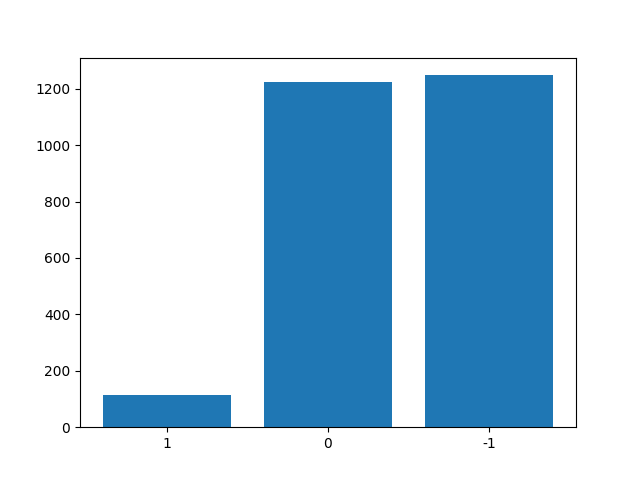
\includegraphics[scale=0.8]{fig_classes}
		\caption{Histograma da frequência de tuítes}
		\label{fig:classes}
	\end{figure}
\end{center}

Pode-se observar nas figura \ref{fig:classes} e tabela \ref{tab:distribution} 
que , ao passo em que as classes negativa e neutra possuem distribuição próxima (48,26\% e 47,29\% 
respectivamente), a classe positiva corresponde a apenas 4,45\% de todos os tuítes. No final da seção
\ref{sec:first_experiments} será visto que esse desbalanceamento entre as classes acarretará um 
desempenho ruim dos classificadores, sejam os desenvolvidos para este trabalho quanto os do
\texttt{scipy}.

\subsection{Características dos tuítes de cada classe}

A fim de entender como os classificadores realizariam o treinamento, analisou-se o conjunto de
dados a procura de padrões de características para cada classe.

Para os tuítes avaliados como neutro, notou-se o padrão que são tuítes derivados de portais de 
notícias ou são indagações, porém sem nenhuma crítica feita nelas.
A tabela abaixo mostra como exemplo alguns tuítes avaliados como neutro.

\begin{center}
	\begin{tabular}{| l | p{0.8\linewidth} |}
		\hline
		usuário & tuíte \\
		\hline
		Tica_Fernandes & Cidades têm protestos contra reforma da Previdência e terceirização http://g1.globo.com/politica/noticia/cidades-tem-protestos-contra-reforma-da-previdência-e-terceirizacao.ghtml \\
		\hline
		andrcolett & Transposição do rio São Francisco, reforma do ensino médio/ da previdência , operação carne fraca, terceirização ... Enem vai bombar esse ano \\
		\hline
		VictoorAugustoo & Via @estadao : Manifestantes protestam em capitais do País contra reforma da Previdência e terceirização - http:/ln.is/estadão.com.brb29w1 \\
		\hline
		EdmilsonPequeno & O meu deputado @luizcoutopt votou contra a terceirização e é contra a reforma da previdência \\
		\hline
	\end{tabular}
\end{center}

Já para os tuítes negativos, nota-se a presença de palavrões e xingamentos 
junto de \textit{hashtags} de teor negativo como por exemplo \#ForaTemer,
além disso é comum a presença de tuítes onde as pessoas são convocadas para manifestações.
Outros termos comuns são escravidão e retrocesso, referindo-se diretamente às reformas da previdência e terceirização.

\begin{center}
	\begin{tabular}{| l | p{0.8\linewidth} |}
		\hline
		usuário & tuíte \\
		\hline
		MgracaGalvao & Dória é o maior Fake de todos os tempos. Se f... Palhaço \\
		\hline
		adamastaquio & Acorda POVO trabalhador. Previdencia + Terceirização + Reforma da CLT é P*** NO RABO DO POVO! \#ReformaTrabalhistaNÃO \\
		\hline
		TheMairaBastos & Reforma da previdência , desmonte da CLT, terceirização ,congelamento de gastos com a saúde e educação \#ForaTemerLadrao \#TemerGolpista \\
		\hline
		neyeverest & O PT esteve no poder por 14 anos o bandido do Lula e a burra da Dilma e o país está um caos pela instituição a roubalheira deles também !! \\
		\hline
		carinasotero & GREVE GERAL DIA 28/04 CONTRA RETROCESSOS DE TEMER • Reforma da Previdência • Reforma Trabalhista • Terceirização irrestrita \\
		\hline
	\end{tabular}
\end{center}

Assim como para os tuítes classificados como negativo, os tuítes positivos também são 
caracterizados pela presença de \textit{hashtags}, sejam elas declarando apoio a um candidato
(como \#Aecio2018 ou \#Lula2018) ou simplesmente manifestando alguma opinião positiva. 

\begin{center}
	\begin{tabular}{| l | p{0.8\linewidth} |}
		\hline
		usuário & tuíte \\
		\hline
		Verinha_Lu & É Aécio pelo Brasil !!! \#AécioPresidenteDoBrasil2018 \#EstamosComAécio \#DeusÉmaior e \#VitóriaVem \#FÉ \#SouAécio \\
		\hline
		Haddad_Femando & O salário mínimo aumentou 71\% durante os governos Lula e Dilma \#BrasilQueOPovoQuer \\
		\hline
		rovisacro & A favor da terceirização e tmb da reforma da previdência ! Mas óbvio, de forma justa e igualitária para todos, principalmente na previdência \\
		\hline	
	\end{tabular}
\end{center}

\section{Descrição dos experimentos}

Realizou-se duas etapas de experimentos, uma primeira etapa utilizando todas as classes onde se
observou que a baixa quantidade de elementos da classe positiva acabava por atrapalhar o desempenho
geral dos algoritmos, em especial os que utilizavam a abordagem OVA para o caso de multiclasses.
Com isso, decidiu-se descartar esses elementos e rodar uma nova sequência de experimentos 
considerando apenas as classes negativa e neutra (que para efeito dos algoritmos será a classe 
positiva) e, com isso, verificar a melhoria dos algoritmos nas métricas.

Para ambas as etapas, procurou-se não só medir o desempenho dos algoritmos, mas também encontrar
uma escolha certa de parâmetros para os mesmos que obtivesse a melhor performance (como a escolha
do Kernel no caso do SVM ou a constante de regularização usada tanto no SVM quanto na regressão
logística).

Tais testes de escolha de parâmetro, caso feitos usando apenas a divisão do conjunto de dados entre
conjunto de treino e conjunto de testes acabaria por dar uma escolha enviesada de parâmetros, uma
vez que uma escolha de parâmetros que tenha bons números em determinado conjunto de testes não
indica que ele possui uma boa generalização, isto é, apresentará uma boa precisão para novos dados.

A fim de garantir maior generalização, utiliza-se um método de validação chamado de 
validação cruzada, que se consiste de um modo de dividir o conjunto de dados e testá-lo com
um conjunto de validação. Uma primeira abordagem da validação cruzada seria dividir nosso conjunto
em três: um de treino, um de validação e outro de teste, assim testaríamos as escolhas de parâmetros
no conjunto de validação e, por fim, mediríamos a performance do melhor no conjunto de teste.

Outra abordagem seria ainda manter a divisão do conjunto de dados em conjunto de treino e teste
porém realizar esse procedimento diversas vezes alternando as porções que irão corresponder a
cada conjunto. Tal método é chamado de k-fold. No k-fold divide-se o conjunto total em k partições
e, a cada iteração, é construído um conjunto de teste usando uma das partições enquanto as k-1
serão o de treino. O procedimento de treinamento é realizado k vezes e, a escolha de parâmetros
com melhor desempenho médio será a escolhida. A figura \ref{fig:kfold} mostra o funcionamento do
método.

\begin{figure}[H]
	\begin{center}
		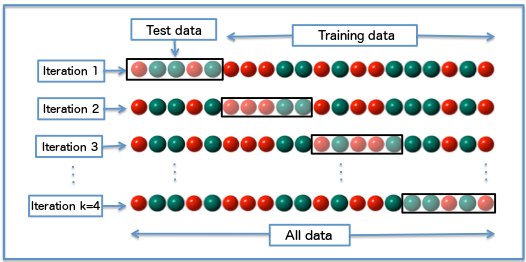
\includegraphics[scale=0.8]{K-fold_cross_validation}
	\end{center}		
	\caption{Funcionamento do método k-fold da validação cruzada \\
		fonte: \url{https://en.wikipedia.org/wiki/Cross-validation_(statistics)\#/media/File:K-fold_cross_validation_EN.jpg}}
	\label{fig:kfold}
\end{figure}

Outro procedimento que foi analisado nos experimentos é se as diferentes escolhas de vetorização afetam
as métricas (ver \ref{subsec:metrics}), todavia esse procedimento de vetorização é feito antes 
do treinamento dos modelos e portanto não foi variado no procedimento de Cross-Validation. 
Em \ref{sec:first_experiments} e \ref{sec:second_experiments} 
os resultados são separados por vetorização e, ao fim de cada rodada, explica-se os resultados 
observados.

O fluxo da realização dos experimentos é descrita no diagrama abaixo:

\begin{figure}[H]
\label{fig:diagram}
	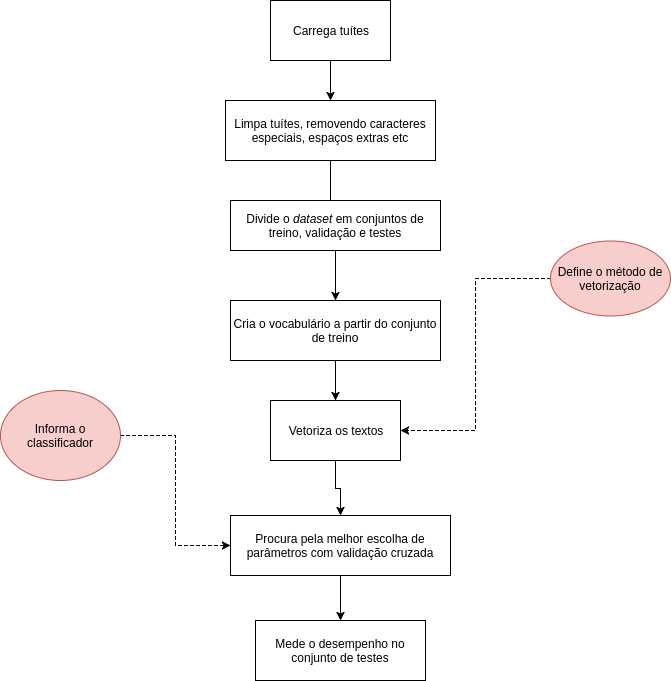
\includegraphics[scale=0.5]{experimento_flow}
	\caption{Passos dos experimentos}
\end{figure}

\subsection{Parâmetros avaliados}
\label{subsec:parameters}

\textbf{SVM}

Para o SVM, testou-se o desempenho do algoritmo com diferentes kernels e com diferentes
parâmetros para cada um. Os seguintes kernels foram utilizados:

\begin{itemize}
	\item Kernel Linear: $K(x, y) = x^Ty$
	\item Kernel RBF: $K(x, y) = exp(-\gamma||x - y||^2)$
	\item Kernel Polinomial: $K(x, y) = (x^Ty + c)^d$
\end{itemize}

Em comum a todos os kernels, variou-se o parâmetro C do SVM utilizado para penalizar os valores
mal classificados. Já para o RBF, varia-se o parâmetro $\gamma$. Por último para o polinomial,
varia-se tanto o parâmetro d que determina o grau do polinômio (aqui variamos entre 3, 4 e 5) e o coeficiente.

\textbf{Regressão Logística}

Para a regressão logística, adicionamos um parâmetro extra $\lambda$ que será usado para penalizar
nosso vetor de pesos e assim, evitar \textit{overfitting}, que ocorre quando um modelo apresenta
baixo erro no conjunto de treino, porém baixa generalização. 
Importante ressaltar que $\lambda$ só é aplicado nos índices
de $1$ a $m + 1$ do vetor de pesos, com o valor do termo $w_0$ não sendo penalizado.


\subsection{Métricas avaliadas}
\label{subsec:metrics}

Para a realização dos experimentos, levou-se em consideração quatro métricas
para avaliar a eficiência dos classificadores.

\begin{itemize}
	\item Acurácia: taxa calculada pela quantidade de dados corretamente classificados
	sobre o total de dados. Quanto mais próximo de 1, melhor.
	\item Precisão: taxa calculada pela expressão $\frac{tp}{tp + fp}$ onde tp corresponde
	aos verdadeiro positivos, isto é, elementos corretamente classificados como da classe C
	e fp são elementos erroneamente classificados na classe C. Uma classe ter precisão alta
	significa que possui um baixo número de amostras classificadas erroneamente nela.
	\item Revocação: taxa calculada pela expressão $\frac{tp}{tp + fn}$ onde tp corresponde
	aos verdadeiro positivos, como na precisão e fn corresponde
	aos falso negativos, isto é, os elementos incorretamente classificados como não pertencentes
	a uma classe C quando na verdade pertencem. Uma alta revocação indica que muitos elementos
	de determinada classe foram corretamente classificados como pertencentes a ela.
	\item Pontuação F1: pode ser interpretado como uma média harmônica entre precisão e revocação é dado
	pela expressão: $2*\frac{precis*revocação}{precis + revocação}$. Assim como as demais medidas, quanto
	mais próximo de 1, melhor o valor.
\end{itemize}

\section{Primeira rodada de experimentos}
\label{sec:first_experiments}

Nesse primeiro experimento, avaliou-se o desempenho dos classificadores desenvolvidos quanto dos
já disponíveis pela biblioteca \texttt{scikit} a fim de comparar o desempenho das implementações.
Além disso, testou-se diferentes escolhas de parâmetro para cada abordagem de vetorizar o corpus
que no caso foram vetor binário, vetor de frequência e vetor com os valores TF-IDF conforme descrito
em \ref{subsec:featurization}. 
Note que neste primeiro experimento, todos os dados foram tratados \textit{in-natura}, sem nenhum método de seleção de características ou qualquer abordagem semelhante a fim de melhorar o desempenho.

\subsection{Implementações próprias}

Dos algoritmos desenvolvidos neste trabalho, testou-se o SVM variando o valor de C entre valores
do intervalo $[10^{-2}, 10^5]$, kernels polinomial, RBF e linear. Para o kernel polinomial foi utilizado
polinômios de grau 3, 4 e 5 e coeficientes 1, 10 e 100. Para o kernel RBF testou valores de $\gamma$
dentro do intervalo $[10^{-9}, 10^3]$. Para cada escolha de vetorização, será colocado apenas os
melhores resultados para cada kernel.

\textbf{Frequência}

\begin{table}[H]
	\centering
	\caption{Resultados para o SVM}
	\begin{tabular}{l l l l}
		\hline
		Kernel & C & parâmetros & Acurácia média \\
		\hline
		Linear & 0,1 & & 0,678 \\
		\hline
		Linear & 1 & & 0,651 \\
		\hline
		RBF & 1 & $\gamma = 0,1$ & 0,683 \\
		\hline
		RBF & $10^5$ & $\gamma = 4,64*10^{-7}$ & 0,678 \\
		\hline
	\end{tabular}
\end{table}

A escolha de parâmetros que obteve maior classificação foi o kernel RBF com C = 1 e $\gamma = 0,1$
com acurácia média de 68,3\%. Usando o classificador com estes parâmetros no conjunto de testes
obteve-se o seguinte resultado:

\begin{table}[H]
	\centering
	\begin{tabular}{l | l | l | l | l}
		\hline
		classe  	&	precisão  &  revocação &  f1\-score &  support \\
		\hline
         -1   &    0.65  &    0.66   &   0.66   &    306 \\
         \hline
          0   &    0.64   &   0.69   &   0.67    &   311 \\
          \hline
          1   &    1.00   &   0.03   &   0.06    &    30 \\
		\hline
		média / total   &    0.67   &   0.65   &   0.64   &    647 \\
		\hline
	\end{tabular}
\end{table}

\textbf{Vetor binário}

\begin{table}[H]
	\centering
	\caption{Resultados para o SVM}
	\begin{tabular}{l l l l}
		\hline
		Kernel & C & parâmetros & Acurácia média \\
		\hline
		Linear & 0,146 & & 0,675 \\
		\hline
		Linear & 0,563 & & 0,658 \\
		\hline
		RBF & 2,154 & $\gamma = 0,1$ & 0,677 \\
		\hline
		RBF & 464,16 & $\gamma = 4,64*10^{-7}$ & 0,676 \\
		\hline
		Polinomial & 0,01 & $c = 1$, $d = 3$ & 0,641 \\
		\hline
		Polinomial & 0,01 & $c = 1$, $d = 3$ & 0,642 \\
		\hline
	\end{tabular}
\end{table}

Como melhor escolha de parâmetros, tivemos o kernel RBF com C = 464,16 e $\gamma = 0,1$ com
67,7\% de acurácia. Utilizando os parâmetros no conjunto de testes, obteve-se os seguintes
resultados:

\begin{table}[H]
	\centering
	\begin{tabular}{l | l | l | l | l}
		\hline
		classe  	&	precisão  &  revocação &  f1\-score &  support \\
		\hline
         -1   &    0.69  &    0.72   &   0.70   &    307 \\
         \hline
          0   &    0.70   &   0.72   &   0.71    &   315 \\
          \hline
          1   &    1.00   &   0.08   &   0.15    &    25 \\
		\hline
		média / total   &    0.71   &   0.70   &   0.69   &    647 \\
		\hline
	\end{tabular}
\end{table}

\textbf{TF-IDF}

\begin{table}[H]
	\centering
	\caption{Resultados para o SVM}
	\begin{tabular}{l l l l}
		\hline
		Kernel & C & parâmetros & Acurácia média \\
		\hline
		Linear & 0,146 & & 0,651 \\
		\hline
		Linear & 0,563 & & 0,664 \\
		\hline
		RBF & 1778,279 & $\gamma = 2,15*10^{-4}$ & 0,667 \\
		\hline
		RBF & 26101,572 & $\gamma = 10^{-5}$ & 0,666 \\
		\hline
		Polinomial & 0,038 & $c = 1$, $d = 4$ & 0,660 \\
		\hline
		Polinomial & 0,147 & $c = 1$, $d = 3$ & 0,663 \\
		\hline
	\end{tabular}
\end{table}

Assim como as demais escolhas de vetorização, a melhor escolha de kernel foi o RBF.
Com valor de C = 1778,279 e $\gamma = 2,15*10^{-4}$ conseguiu-se acurácia média de 66,7\%.
Utilizando esse classificador no conjunto de testes, obtiveram-se os seguintes resultados:

\begin{table}[H]
	\centering
	\begin{tabular}{l | l | l | l | l}
		\hline
		classe  	&	precisão  &  revocação &  f1\-score &  support \\
		\hline
         -1   &    0.68  &    0.73   &   0.70   &    322 \\
         \hline
          0   &    0.67   &   0.69   &   0.68    &   296 \\
          \hline
          1   &    1.00   &   0.03   &   0.07    &    29 \\
		\hline
		média / total   &    0.69   &   0.68   &   0.66   &    647 \\
		\hline
	\end{tabular}
\end{table} 

Pelos resultados dos experimentos, tivemos que a melhor escolha de classificador e vetorização
foi o kernel RBF com vetorização por frequência com 68,3\% de acurácia. Ao observarmos as outras
métricas, percebemos que os valores médios para precisão, revocação e pontuação f1 estão razoáveis,
entretanto ao olharmos para os valores de revocação e pontuação f1 da classe positiva, vemos
que estes são quase 0 ao passo que a precisão é 1. Isso indica que apenas poucos elementos foram
colocados nesta classe corretamente e nenhum foi colocado incorretamente, porém a maioria dos
elementos desta classe foram marcados nas demais classes.

Tais valores para classe positiva são devidos à baixa quantidade de dados da mesma, o que acaba
prejudicando o desempenho do classificador que separa esta classe das demais.

Utilizou-se o melhor classificador para verificar alguns tuítes mal classificados e entender melhor
o funcionamento do classificador.

\begin{table}[H]
	\centering	
	\begin{tabular}{| p{0.8\linewidth} | l | l |}
		\hline
		Tuíte & Previsto & Real \\
		O cara tá falando da terceirização anta. Eu sou contra essa reforma da previdência deste jeito, ela deve ser revista.A trabalhista eu apoio & -1 &  1 \\
		\hline
		Ops @MichelTemer não tem um papel com os trabalhadores e a lei da terceirização assim fala os especialistas imagina essa REFORMA PREVIDÊNCIA  http://pic.twitter.com/KjLa26TCwy &  -1 & 0 \\
		\hline
		A agenda do Lula para os próximos meses está lotada... de depoimentos em processos em que ele é réu. http://owl.li/F3Ij30flUaY & 0 & -1 \\
		\hline
		Contra reforma da Previdência e terceirização ... http://fb.me/18guG6FGR & 0 & -1 \\
		\hline
		Não podemos discutir a Reforma da Previdência sem discutir a Terceirização e outros elementos desse desmonte de direitos", Ruy (APLB)" & -1 & 0 \\
		\hline
		Muso inspirador da presidenta Dilma ! & 0 & 1 \\
		\hline
	\end{tabular}
\end{table} 

Para os tuítes negativos que foram erroneamente classificados, percebemos que o classificador os
colocou na classe neutra pela maior presença de palavras encontradas em tuítes de notícias, no segundo
caso percebe-se que há uma ambiguidade no tuíte e, enquanto foi classificado com negativo, poderia
ter sido também classificado como neutro por outra pessoa.

Na classe neutra, temos que em um há uma ambiguidade no tuíte e não possui informação suficiente
para avaliar sua polaridade, porém no segundo caso pode-se dizer que o tuíte foi classificado corretamente
pois o classificador levou em conta que chamou a reforma de previdência e a terceirização de desmonte
de direitos, apesar de o tuíte em si apenas relatar o que foi dito.

Para a classe positiva notou-se dois casos: em um a presença de um xingamento colocou o tuíte como
opinião negativa e no outro caso o classificador interpretou o tuíte como uma simples constatação
de fatos.


\subsection{Implementações do \texttt{scikit}}

Abaixo, separaremos os testes baseados em como a obtenção do vetor de \textit{features} foi feita
ao invés dos algoritmos, uma vez que para todos esses realizou-se os mesmos testes. Importante 
ressaltar que só serão colocados aqui os melhores resultados de cada um, uma vez que existe uma
grande quantidade de resultados. 

Os resultados dos experimentos serão comentados apenas ao final desta subseção, após mostrar
os valores encontrados para todas as formas de vetorização.


\textbf{Frequência}

\begin{table}[H]
	\centering
	\caption{Resultados para o SVM}
	\begin{tabular}{l l l l}
		\hline
		Kernel & C & parâmetros & Acurácia média \\
		\hline
		Linear & 0,1 & & 0,666 \\
		\hline
		Linear & 1 & & 0,637 \\
		\hline
		RBF & 100 & $\gamma = 10^{-3}$ & 0,663 \\
		\hline
		RBF & 100 & $\gamma = \frac{1}{\# amostras}$ & 0,653 \\
		\hline
		Polinomial & 0,01 & $c = 10$, $d = 5$ & 0,666 \\
		\hline
		Polinomial & 100 & $c = 1$, $d = 4$ & 0,663 \\
		\hline
	\end{tabular}
\end{table}

Importante ressaltar que em casos de empate, o primeiro melhor será selecionado, no caso o melhor
foi o kernel linear com $C = 0.1$, utilizando esses valores no conjunto de testes obtiveram-se os 
seguintes resultados:

\begin{table}[H]
	\centering
		\begin{tabular}{l | l | l | l | l}
		\hline
		classe  	&	precisão  &  revocação &  f1\-score &  support \\
		\hline		
		 -1     &  0.70  &    0.73   &   0.71   &    324 \\
		  \hline
          0     &  0.67   &   0.69   &   0.68    &   298 \\
          \hline
          1     &  1.00   &   0.04   &   0.08    &    25 \\
			\hline
		média / total     &  0.70  &    0.68  &    0.67   &    647 \\
		\hline
	\end{tabular}
\end{table}

Para a regressão logística, variou-se o valor de $\lambda$ entre $10^{-4}$ a $1$ e, além disso
variou-se a abordagem para o caso multiclasses, uma vez que o \texttt{scikit} disponibiliza
uma implementação usando o método OVA e outro usando o método multinomial (assim como implementou-se).

\begin{table}[H]
	\centering
	\caption{Resultados da regressão logística}
	\begin{tabular}{l l l}
		\hline
		Método & $\lambda$ & Acurácia média \\
		\hline
		OVA & 0.1 & 0.654 \\
		\hline
		OVA & 1 & 0.651 \\
		\hline
		Multinomial & 0.1 & 0.654 \\
		\hline
		Multinomial & 1 & 0.649 \\
		\hline
	\end{tabular}
\end{table}

Assim como para o SVM, escolheu-se o primeiro melhor que no caso é a abordagem OVA com $\lambda = 0.1$.
Deu os seguintes resultados no conjunto de testes:

\begin{table}[H]
	\centering
		\begin{tabular}{l | l | l | l | l}
		\hline
		classe  	&	precisão  &  revocação &  f1\-score &  support \\
		\hline
         -1   &    0.70  &    0.68   &   0.69   &    320 \\
         \hline
          0    &   0.68   &   0.73   &   0.70   &    307 \\
          \hline
          1    &   0.50   &   0.15   &   0.23   &     20 \\
		\hline
		média / total  &     0.68  &    0.69    &  0.68   &    647 \\
		\hline
	\end{tabular}
\end{table}

\textbf{Vetor binário}

\begin{table}[H]
	\centering
	\caption{Resultados para o SVM}
	\begin{tabular}{l l l l}
		\hline
		Kernel & C & parâmetros & Acurácia média \\
		\hline
		Linear & 0,1 & & 0,658 \\
		\hline
		Linear & 1 & & 0,643 \\
		\hline
		RBF & 100 & $\gamma = 10^{-3}$ & 0,649 \\
		\hline
		RBF & 100 & $\gamma = \frac{1}{\# amostras}$ & 0,646 \\
		\hline
		Polinomial & 100 & $c = 1$, $d = 4$ & 0,656 \\
		\hline
		Polinomial & 1 & $c = 5$, $d = 4$ & 0,658 \\
		\hline
	\end{tabular}
\end{table}

Assim como para o vetor de frequências, a melhor escolha de parâmetros encontrada na validação
cruzada foi C = 0,1 e kernel linear. Executando no conjunto de testes obtiveram-se os seguintes
resultados:

\begin{table}[H]
	\centering
		\begin{tabular}{l | l | l | l | l}
		\hline
		classe  	&	precisão  &  revocação &  f1\-score &  support \\
		\hline
         -1    &   0.66   &   0.76  &    0.71    &   310 \\
         \hline
          0     &  0.69   &   0.66   &   0.67    &   302 \\
         \hline
          1     &  1.00  &    0.06   &   0.11    &    35 \\
		\hline
		média / total    &   0.69   &   0.68   &   0.66    &   647 \\
		\hline
	\end{tabular}
\end{table}

\begin{table}[H]
	\centering
	\caption{Resultados da regressão logística}
	\begin{tabular}{l l l}
		\hline
		Método & $\lambda$ & Acurácia média \\
		\hline
		OVA & 0.1 & 0.631 \\
		\hline
		OVA & 1 & 0.634 \\
		\hline
		Multinomial & 0.1 & 0.631 \\
		\hline
		Multinomial & 1 & 0.630 \\
		\hline
	\end{tabular}
\end{table}

Tal qual com o vetor de frequências, escolheu-se a abordagem OVA e $\lambda = 1$ obtendo os seguintes
resultados no conjunto de testes:

\begin{table}[H]
	\centering
		\begin{tabular}{l | l | l | l | l}
		\hline
		classe  	&	precisão  &  revocação &  f1\-score &  support \\
		\hline
		 -1    &   0.68   &   0.73  &    0.71   &    305 \\
		 \hline
          0    &   0.70   &   0.69   &   0.69   &    317 \\
          \hline
          1   &    0.33   &   0.04   &   0.07   &     25 \\
		 \hline
		média / total    &   0.67   &   0.69  &    0.68   &    647 \\
		\hline
	\end{tabular}
\end{table}

\textbf{TF-IDF}

\begin{table}[H]
	\centering
	\caption{Resultados para o SVM}
	\begin{tabular}{l l l l}
		\hline
		Kernel & C & parâmetros & Acurácia média \\
		\hline
		Linear & 1 & & 0,658 \\
		\hline
		Linear & 10 & & 0,627 \\
		\hline
		RBF & 100 & $\gamma = 10^{-3}$ & 0,651 \\
		\hline
		RBF & 1 & $\gamma = 10^{-4}$ & 0,483 \\
		\hline
		Polinomial & 1 & $c = 5$, $d = 5$ & 0,678 \\
		\hline
		Polinomial & 10 & $c = 10$, $d = 3$ & 0,677 \\
		\hline
	\end{tabular}
\end{table}

Com essa vetorização, diferente das demais, os melhores parâmetros escolhidos foram kernel polinomial
com coeficiente e grau 5. Utilizando esses valores, obtiveram-se o seguinte resultado no conjunto de
testes:

\begin{table}[H]
	\centering
		\begin{tabular}{l | l | l | l | l}
		\hline
		classe  	&	precisão  &  revocação &  f1\-score &  support \\
		\hline
		 -1    &   0.64   &   0.79   &   0.71   &    311 \\
		 \hline
          0    &   0.69   &   0.60  &    0.64    &   301 \\
          \hline
          1   &    0.00   &   0.00   &   0.00    &    35 \\
          \hline
		média / total   &    0.63   &   0.66   &   0.64   &    647 \\
		\hline
	\end{tabular}
	\caption{Métricas para o melhor classificador do \texttt{scikit} no caso de três classes}
	\label{tab:best_scikit}
\end{table}

\begin{table}[H]
	\centering
	\caption{Resultados da regressão logística}
	\begin{tabular}{l l l}
		\hline
		Método & $\lambda$ & Acurácia média \\
		\hline
		OVA & 0.1 & 0.659 \\
		\hline
		OVA & 1 & 0.665 \\
		\hline
		Multinomial & 0.1 & 0.660 \\
		\hline
		Multinomial & 1 & 0.662 \\
		\hline
	\end{tabular}
\end{table}

Neste teste, assim como os demais usando a regressão logística, escolheu-se a abordagem OVA com
$\lambda = 1$ obtendo seguintes resultados no conjunto de testes:

\begin{table}[H]
	\centering
		\begin{tabular}{l | l | l | l | l}
		\hline
		classe  	&	precisão  &  revocação &  f1\-score &  support \\
		\hline
		 -1    &   0.66   &   0.75   &   0.70   &    312 \\
		 \hline
          0    &   0.69   &   0.66   &   0.68   &    310 \\
          \hline
          1    &   0.00   &   0.00   &   0.00    &    25 \\
		\hline
		média / total   &    0.65   &   0.68   &   0.66   &    647 \\
		\hline
	\end{tabular}
\end{table}

Observa-se que, para ambos os algoritmos tem-se que nenhum valor foi classificado como
positivo quando usou-se a vetorização através do valor TF-IDF de cada termo, apesar de ainda
apresentar desempenho médio aceitável. 

Isso se deve ao fato de vetorização por TF-IDF
leva-se em consideração a relevância das palavras na sentença como um todo e, possivelmente
algumas palavras associadas a documentos positivos estão também associadas
a documentos neutros e, consequentemente, não possuem um valor TF-IDF alto, aliado ao fato de o vocabulário
ser montado levando em conta apenas as 5000 palavras com melhores pontuações ou presença, portanto
algumas palavras explicitamente associadas a documentos positivos não compuseram o vetor de
\textit{features}.

Por outro lado se olharmos os desempenhos utilizando frequências simples ou um vetor binário
obtemos resultados semelhantes para ambos os algoritmos, todavia ainda existe um melhor desempenho
com a vetorização por frequências tal como o SVM apresenta melhores resultados em relação à regressão
logística, mesmo que com pouca diferença.

Assim como o outro classificador, analisou-se os tuítes classificados incorretamente a fim de
entender o funcionamento do classificador:

\begin{table}[H]
	\centering
	\begin{tabular}{| p{0.8\linewidth} | l | l |}
		\hline
		Tuíte & Previsto & Real \\
		\hline
		Lula ainda lidera as pesquisas oficiais em todo o Brasil & -1 & 0 \\
		\hline
		Sem querer ser chata, mas foi a Dilma quem começou com os Projetos de Reforma da Previdência e de Terceirização & -1 & 0 \\
		\hline
		simm, e irei, quero a reforma da previdência , a terceirização , reforma da CLT, tudo isso p o Brasil voltar a crescer :) & -1 & 1 \\
		\hline
		O cara tá falando da terceirização anta. Eu sou contra essa reforma da previdência deste jeito, ela deve ser revista.A trabalhista eu apoio & -1 & 1 \\
		\hline
		Temer não é santo,mas não entender o conceito que deu uma freada na beira do abismo que Lula Dilma estavam nos empurrando é DESINFORMAÇÃOhttps://twitter.com/Acppprovesi/status & 0 & -1 \\
		\hline
		Texto: Os alunos da FDCE se posicionam CONTRA a reforma da previdência , trabalhista e a terceirização ! Quem é de luta e... http://fb.me/1YA1jro5z & 0 & -1 \\
		\hline
	\end{tabular}
\end{table}

Observa-se na tabela, assim como para as implementações próprias, houve a classificação errada
de tuítes positivos como negativos devida à presença de xingamentos no tuíte. Além disso tuítes
negativos costumam ser classificados erroneamente como neutros pelo texto se assemelhar com uma
constatação de um fato, mesmo que possua a presença de termos negativos.

Comum a todos os experimentos foram resultados ruins associados à classe positiva. No caso do SVM
obtiveram-se alta precisão em alguns casos, porém as taxas de revocação e f1-score foram baixas. Valores
baixos para revocação e f1-score podem ser interpretados como um sinal de que os classificadores
são ruins para detectar opiniões positivas. A exemplo do melhor classificador, tem-se uma taxa
de revocação de 0,08 que indica que 92\% das amostras positivas não são detectadas pelo algoritmo.

Motivado pelo baixo desempenho visto na classe positiva em todos os experimentos aliado à baixa
quantidade de tuítes nessa classe, rodou-se mais experimentos, porém dessa vez usando apenas as
outras classes.

\section{Segunda rodada de experimentos}
\label{sec:second_experiments}

Nesta segunda rodada de experimentos, removeu-se os elementos pertencentes à classe positiva.
Assim como na primeira rodada, testou-se diferentes escolhas de parâmetros para cada um dos
algoritmos e testou-se com os dados \textit{in natura}. Como viu-se na primeira rodada de experimentos
que havia pouca diferença entre a vetorização por frequência e presença do termo, optou-se por testar
apenas usando frequência e TF-IDF.

\subsection{Implementações próprias}

Para as implementações próprias do SVM, testou-se os kernels polinomial, linear e RBF alternando
diversos parâmetros destes. Assim como na rodada anterior, só será mostrado aqui os melhores resultados
obtidos. 

\textbf{Frequência}

\begin{table}[H]
	\centering
	\caption{Resultados para o SVM}
	\begin{tabular}{l l l l}
		\hline
		Kernel & C & parâmetros & Acurácia média \\
		\hline
		Linear & 0,1 & & 0,679 \\
		\hline
		Linear & $10^{10}$ & & 0,667 \\
		\hline
		RBF & 1 & $\gamma = 0,1$ & 0,698 \\
		\hline
		RBF & 10 & $\gamma = 0,1$ & 0,697 \\
		\hline
		Polinomial & 0,1 & $c = 10^{-4}$, $d = 3$ & 0,679 \\
		\hline
		Polinomial & 100 & $c = 10^{-4}$, $d = 5$ & 0,679 \\
		\hline
	\end{tabular}
\end{table}

Nesta rodada, escolheu-se usar o kernel RBF com $\gamma = 0,1$ e C = 1 que obteve 69,8\% de acurácia média. No
conjunto de testes teve os seguintes resultados:

\begin{table}[H]
	\centering
		\begin{tabular}{l | l | l | l | l}
		\hline
		classe  	&	precisão  &  revocação &  f1-score &  support \\
		\hline
		 -1    &   0.73   &   0.62   &   0.67   &    343 \\
		 \hline
          0    &   0.60   &   0.71   &   0.65   &    275 \\
		\hline
		média / total   &    0.67   &   0.66   &   0.66   &    618 \\
		\hline
	\end{tabular}
\end{table}


\begin{table}[H]
	\centering
	\caption{Resultados da regressão logística}
	\begin{tabular}{l l}
		\hline
		$\lambda$ & Acurácia média \\
		\hline
		$10^{-5}$ & 0,637 \\
		\hline
		0,316 & 0,684 \\
		\hline
		$10^{4}$ & 0,544 \\
	\end{tabular}
\end{table}

Utilizando então $\lambda = 0,316$ foi obtido 68,4\% de acurácia média e, ao utilizar
o classificador no conjunto de testes teve os seguintes resultados:

\begin{table}[H]
	\centering
		\begin{tabular}{l | l | l | l | l}
		\hline
		classe  	&	precisão  &  revocação &  f1-score &  support \\
		\hline
		 -1    &   0.68   &   0.69   &   0.68   &    301 \\
		 \hline
          0    &   0.70   &   0.69   &   0.69   &    317 \\
		\hline
		média / total   &    0.69   &   0.69   &   0.69   &    618 \\
		\hline
	\end{tabular}
\end{table}

\textbf{TF-IDF}

\begin{table}[H]
	\centering
	\caption{Resultados para o SVM}
	\begin{tabular}{l l l l}
		\hline
		Kernel & C & parâmetros & Acurácia média \\
		\hline
		Linear & 0,1 & & 0,688 \\
		\hline
		Linear & 1 & & 0,697 \\
		\hline
		RBF & 1 & $\gamma = 1$ & 0,704 \\
		\hline
		RBF & $10^{9}$ & $\gamma = 1$ & 0,700 \\
		\hline
		Polinomial & 1 & $c = 10^{-4}$, $d = 3$ & 0,697 \\
		\hline
		Polinomial & 1 & $c = 10^{-4}$, $d = 5$ & 0,697 \\
		\hline
	\end{tabular}
\end{table}

Os melhores parâmetros para esta rodada de testes foi o kernel RBF com $\gamma$ e C valendo 1 que
obteve acurácia média de 70,4\%. Utilizando estes parâmetros no conjunto de testes obtiveram-se os
seguintes valores:

\begin{table}[H]
	\centering
		\begin{tabular}{l | l | l | l | l}
		\hline
		classe  	&	precisão  &  revocação &  f1-score &  support \\
		\hline
		 -1    &   0.69   &   0.79   &   0.74   &    305 \\
		 \hline
          0    &   0.76   &   0.65   &   0.71   &    313 \\
		\hline
		média / total   &    0.73   &   0.72   &   0.72   &    618 \\
		\hline
	\end{tabular}
\end{table}

\begin{table}[H]
	\centering
	\caption{Resultados da regressão logística}
	\begin{tabular}{l l}
		\hline
		$\lambda$ & Acurácia média \\
		\hline
		$10^{-5}$ & 0,662 \\
		\hline
		0,316 & 0,697 \\
		\hline
		$10^{4}$ & 0,585 \\
	\end{tabular}
\end{table}

Assim como na rodada anterior, o melhor parâmetro foi $\lambda = 0,316$, porém desta vez obteve
69,7\% de acurácia. Utilizando este parâmetro de regularização no conjunto de testes obtiveram-se
os seguintes resultados:

\begin{table}[H]
	\centering
		\begin{tabular}{l | l | l | l | l}
		\hline
		classe  	&	precisão  &  revocação &  f1-score &  support \\
		\hline
		 -1    &   0.70   &   0.68   &   0.69   &    323 \\
		 \hline
          0    &   0.66   &   0.67   &   0.67   &    295 \\
		\hline
		média / total   &    0.68   &   0.68   &   0.68   &    618 \\
		\hline
	\end{tabular}
\end{table}

Por fim da rodada de testes com as implementações próprias dos classificadores, chegou
a conclusão de que o algoritmo SVM em conjunto com a vetorização por TF-IDF trouxe um bom
compromisso entre acurácia, precisão e revocação tendo todas as suas médias acima de 70\%
para todas as métricas sendo assim um classificador com alta probabilidade de trazer resultados
relevantes para novos documentos. Além disso o procedimento de validação cruzada garante
que o classificador possui capacidade de generalização, uma vez que realiza o treinamento e
validação com conjuntos diferentes mais de uma vez.

Interessante comentar que ao passo que a regressão logística não chegou a ter
acurácia melhor em nenhuma vetorização, porém ao olharmos para os valores médios de precisão,
revocação e pontuação f1 vemos que, com exceção da melhor versão do SVM, foi superior indicando
que este algoritmo possui robustez ao trazer valores relevantes.

\subsection{Implementações do \texttt{scitkit}}

Para as implementações do \texttt{scikit}, realizou-se os experimentos da mesma forma que
para o caso com três classes com a única diferença sendo os valores para $\gamma$ ao qual
testou o kernel RBF.

\textbf{Frequência}

\begin{table}[H]
	\centering
	\caption{Resultados para o SVM}
	\begin{tabular}{l l l l}
		\hline
		Kernel & C & parâmetros & Acurácia média \\
		\hline
		Linear & 0,1 & & 0,699 \\
		\hline
		Linear & 1 & & 0,680 \\
		\hline
		RBF & 1 & $\gamma = 0,158$ & 0,713 \\
		\hline
		RBF & 10 & $\gamma = 0,158$ & 0,701 \\
		\hline
		Polinomial & 1 & $c = 5$, $d = 4$ & 0,698 \\
		\hline
		Polinomial & 100 & $c = 1$, $d = 4$ & 0,697 \\
		\hline
	\end{tabular}
\end{table}

Como melhor resultado tivemos o kernel RBF com $\gamma = 0,158$ com acurácia média
de 71,3\%. Utilizando essa escolha de parâmetros no conjunto de testes, obtiveram-se
os seguintes resultados:

\begin{table}[H]
	\centering
		\begin{tabular}{l | l | l | l | l}
		\hline
		classe  	&	precisão  &  revocação &  f1-score &  support \\
		\hline
		 -1    &   0.69   &   0.63   &   0.66   &    327 \\
		 \hline
          0    &   0.62   &   0.68   &   0.65   &    291 \\
		\hline
		média / total   &    0.66   &   0.66   &   0.66   &    618 \\
		\hline
	\end{tabular}
\end{table}

\begin{table}[H]
	\centering
	\caption{Resultados da regressão logística}
	\begin{tabular}{l l}
		\hline
		$\lambda$ & Acurácia média \\
		\hline
		$0,1$ & 0,693 \\
		\hline
		1 & 0,696 \\
		\hline
		1000 & 0,676 \\
	\end{tabular}
\end{table}

Como resultado, obtivemos que o melhor valor para $\lambda$ era 1 que nos deu uma acurácia
média de 69,6\% e para o conjunto de testes deu os seguintes resultados:

\begin{table}[H]
	\centering
		\begin{tabular}{l | l | l | l | l}
		\hline
		classe  	&	precisão  &  revocação &  f1-score &  support \\
		\hline
		 -1    &   0.65   &   0.68   &   0.66   &    300 \\
		 \hline
          0    &   0.68   &   0.65   &   0.67   &    318 \\
		\hline
		média / total   &    0.66   &   0.66   &   0.66   &    618 \\
		\hline
	\end{tabular}
\end{table}


\textbf{TF-IDF}

\begin{table}[H]
	\centering
	\caption{Resultados para o SVM}
	\begin{tabular}{l l l l}
		\hline
		Kernel & C & parâmetros & Acurácia média \\
		\hline
		Linear & 1 & & 0,702 \\
		\hline
		Linear & 10 & & 0,676 \\
		\hline
		RBF & 1 & $\gamma = 0,158$ & 0,710 \\
		\hline
		RBF & 100 & $\gamma = 0,00398$ & 0,702 \\
		\hline
		Polinomial & 0,1 & $c = 10$, $d = 5$ & 0,701 \\
		\hline
		Polinomial & 10 & $c = 10$, $d = 4$ & 0,702 \\
		\hline
	\end{tabular}
\end{table}

Como melhor escolha de parâmetros tivemos o kernel RBF com $\gamma = 0,158$ com 71\% de
acurácia média. Testando no conjunto de testes obtiveram-se os seguintes resultados:

\begin{table}[H]
	\centering
		\begin{tabular}{l | l | l | l | l}
		\hline
		classe  	&	precisão  &  revocação &  f1-score &  support \\
		\hline
		 -1    &   0.68   &   0.75   &   0.71   &    326 \\
		 \hline
          0    &   0.68   &   0.61   &   0.65   &    292 \\
		\hline
		média / total   &    0.68   &   0.68   &   0.68   &    618 \\
		\hline
	\end{tabular}
\end{table}

\begin{table}[H]
	\centering
	\caption{Resultados da regressão logística}
	\begin{tabular}{l l}
		\hline
		$\lambda$ & Acurácia média \\
		\hline
		$0,1$ & 0,686 \\
		\hline
		1 & 0,688 \\
		\hline
		10 & 0,671 \\
	\end{tabular}
\end{table}


Com isso temos que a melhor escolha para $\lambda$ é 1 que obteve 68,8\% de acurácia média.
Utilizando este parâmetro para classificar o conjunto de testes, obtiveram-se os seguintes resultados:

\begin{table}[H]
	\centering
		\begin{tabular}{l | l | l | l | l}
		\hline
		classe  	&	precisão  &  revocação &  f1-score &  support \\
		\hline
		 -1    &   0.71   &   0.77   &   0.74   &    313 \\
		 \hline
          0    &   0.74   &   0.68   &   0.71   &    305 \\
		\hline
		média / total   &    0.73   &   0.72   &   0.72   &    618 \\
		\hline
	\end{tabular}
\end{table}

As implementações do \texttt{scikit} apresentaram uma acurácia maior em relação às
desenvolvidas, apesar de a diferença não ser expressiva. Interessante notar que,
ao contrário das implementações próprias, o melhor classificador, no caso o SVM
com kernel RBF e vetorização por frequência não obtiveram os melhores valores para
todas as métricas avaliadas, uma vez que o melhor classificador em termos de
precisão, revocação e pontuação f1 foi a regressão logística usando a vetorização
com TF-IDF, que por sua vez apresentou resultados acima de 70\%.

Percebemos também que a vetorização por TF-IDF acaba sendo melhor para as métricas
de precisão, revocação e pontuação f1, pois todos os classificadores performaram
melhor ao escolher essa vetorização. Isso se deve ao fato de o TF-IDF de um termo
dar maior ênfase aos termos característicos de um documento, facilitando a identificação
de uma entrada que corresponda a um texto neutro ou a um negativo.

\section{Comparação entre experimentos}

Ao fim da última rodada dos experimentos, resolveu comparar os resultados vistos em 
\ref{sec:first_experiments} e \ref{sec:second_experiments} para saber ver as mudanças
efetivas nos resultados com e sem a classe positiva no \textit{dataset}.

Importante ressaltar que nessa comparação serão usados apenas os melhores resultados de
de cada rodada, separando apenas as comparações entre as implementações próprias
e as implementações do \texttt{scikit}.

\subsection{Implementações Próprias}

Nas implementações próprias, comparou-se as duas versões do SVM com kernel RBF
, uma com $\gamma = 0.1$ e $C = 1$ (caso multiclasses) e outra com $C$ e $\gamma$ iguais a 1 (caso 
binário).  

\begin{table}[H]
	\centering
	\begin{tabular}{l l l}
	& Multiclasses & Binário \\
	\hline
	Acurácia Média & 68,3\% & 70,4\% \\
	\hline
	Precisão Média & 0.67 & 0.73 \\
	\hline
	Revocação Média & 0.65 & 0.72 \\
	\hline
	F1-Score Média & 0.64 & 0.72 \\
	\hline
	\end{tabular}
\end{table}

Nas implementações próprias, nota-se melhora significativa ao remover a classe positiva, ao passo
em que todos os valores médios aumentaram em pelo menos 2\% em comparação com o caso multiclasses.
Isso se deve ao fato de que, no caso multiclasses, muitos elementos da classe positiva eram
classificados erroneamente, portanto abaixavam os valores de precisão, revocação e F1-Score médios.

\subsection{Implementações do \texttt{scikit}}

Já para as versões do \texttt{scikit}, comparou-se também duas versões do SVM,
uma com kernel polinomial, $C = 1$ e grau 5 com coeficiente 5 (caso multiclasses) com
outra utilizando o kernel RBF, $C = 1$ e $\gamma = 0.158$ (caso binário).

\begin{table}[H]
	\centering
	\begin{tabular}{l l l}
	& Multiclasses & Binário \\
	\hline
	Acurácia Média & 67,8\% & 71,3\%  \\
	\hline
	Precisão Média & 0.63 & 0.66  \\
	\hline
	Revocação Média & 0.66 & 0.66 \\
	\hline
	F1-Score Média & 0.64 & 0.66 \\
	\hline
	\end{tabular}
\end{table}

Para as implementações do \texttt{scikit}, nota-se que ao passo em que a acurácia média aumentou em
quase 4\%, as demais métricas não obtiveram aumento significativo em relação ao caso de três classes,
porém ao olhar para \ref{tab:best_scikit} observa-se que para a classe positiva não teve nenhum 
elemento atribuído a ela, portanto as médias foram realizadas levando em consideração apenas as duas
classes predominantes, justificando a semelhança de valores com a apresentada no caso binário.
